\documentclass[conference]{IEEEtran}
\usepackage[utf8]{inputenc}
\usepackage[T1]{fontenc}
\usepackage[spanish,es-tabla]{babel}
\usepackage{graphicx}
\usepackage{cite}
\usepackage{url}
% Las figuras están en docs/ (en el repositorio) o junto a main.tex (en Overleaf).
\graphicspath{{./}{../}}
\renewcommand\IEEEkeywordsname{Palabras clave}

\begin{document}

\title{Videojuego multijugador cliente-servidor sobre una red LAN--WAN--LAN}

\author{\IEEEauthorblockN{Martin Pineda Jaramillo, David Felipe Beltran Tabares y Juan David Navarro Bermudez}
\IEEEauthorblockA{Curso de Redes de Computadores\\
Universidad de los Llanos\\
Villavicencio, Colombia}}

\maketitle

\begin{abstract}
Este trabajo presenta el diseño y la implementación de un videojuego de disparos
multijugador en 3D que aplica la arquitectura cliente-servidor sobre una red
formada por dos redes de área local unidas por un enlace WAN entre dos routers.
El juego se desarrolló en Godot 4.7 y usa el protocolo UDP por medio de la
biblioteca ENet. El servidor tiene la autoridad sobre el estado de la partida y
los clientes solo envían sus entradas. La red se diseñó con direccionamiento
privado y rutas estáticas, y se validó en Cisco Packet Tracer, donde cuatro
clientes alcanzan al servidor a través de los dos routers sin pérdida de
paquetes. Una prueba funcional con cinco jugadores simultáneos confirmó la
sincronización del estado, con una latencia de ida y vuelta de 9~ms en un mismo
equipo.
\end{abstract}

\begin{IEEEkeywords}
cliente-servidor, UDP, enrutamiento estático, red LAN, red WAN, Packet Tracer,
videojuego multijugador.
\end{IEEEkeywords}

\section{Introducción}
Los videojuegos multijugador en tiempo real son un buen caso de estudio para un
curso de redes: necesitan baja latencia, deben tolerar la pérdida de paquetes y
obligan a decidir qué equipo tiene la última palabra sobre lo que ocurre en la
partida. Estas decisiones se relacionan de forma directa con los modelos de
comunicación y con los protocolos de la capa de transporte~\cite{kurose}.

El objetivo de este proyecto es demostrar la arquitectura cliente-servidor en
una red que no es plana. La topología exigida es un computador conectado a un
router en una red LAN, ese router conectado a un segundo router por un enlace
WAN, y en el otro extremo una segunda red LAN con los demás computadores. Así,
el tráfico del juego debe ser enrutado entre redes distintas.

El trabajo tiene tres partes: el diseño de la red, la implementación del juego y
la validación, que se hizo con una simulación en Cisco Packet Tracer y con
pruebas funcionales del juego.

\section{Marco teórico}
\subsection{Arquitectura cliente-servidor}
En el modelo cliente-servidor un proceso, el servidor, espera solicitudes en una
dirección y un puerto conocidos, y los clientes inician la
comunicación~\cite{kurose}. En un videojuego, además, el servidor suele ser
autoritativo: es el único que simula la partida, y los clientes le envían lo que
el jugador quiere hacer y dibujan el estado que el servidor les devuelve. Con
esto todos los jugadores ven lo mismo y un cliente no puede alterar su posición
ni su vida~\cite{fiedler}.

\subsection{Protocolo UDP y ENet}
UDP es un protocolo de transporte sin conexión que no retransmite ni ordena los
datagramas~\cite{rfc768}. En un juego esto es una ventaja: una posición que
llega tarde ya no sirve, y esperar su retransmisión, como haría TCP, retrasaría
los datos nuevos~\cite{fiedler}. ENet es una biblioteca que funciona sobre UDP y
añade lo que le falta de forma opcional: conexiones, canales y entrega fiable
solo para los mensajes que la necesitan~\cite{enet}.

\subsection{Direccionamiento y enrutamiento}
Las redes locales usan los rangos de direcciones privadas definidos en el
RFC~1918~\cite{rfc1918}. Un router conoce de forma automática las redes
conectadas a sus interfaces; para llegar a una red remota necesita una ruta, que
puede configurarse a mano (ruta estática) o aprenderse con un protocolo de
enrutamiento. En una red de dos routers la ruta estática es la opción más
simple~\cite{kurose}.

\section{Diseño de la red}
La Fig.~\ref{fig:topologia} muestra la topología. En la LAN~A hay un solo
computador, que crea la partida y actúa como servidor y como jugador. En la
LAN~B están los demás jugadores, que se conectan como clientes. Cada LAN tiene
un switch y un router, y los routers se unen por un enlace que representa la
WAN. No se usa un servidor dedicado ni servicios externos: todo es local.

\begin{figure*}[t]
\centering
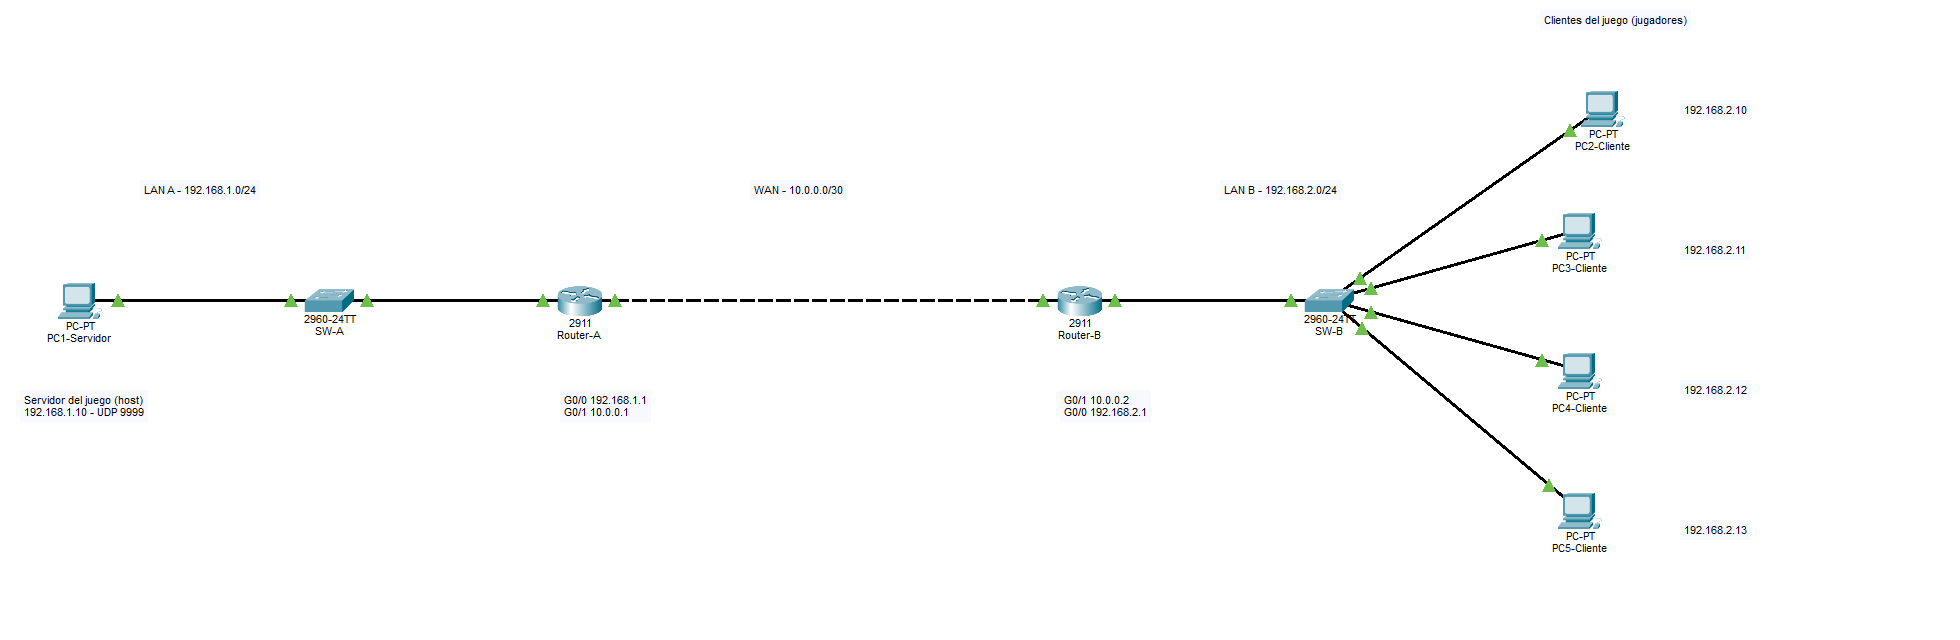
\includegraphics[width=0.9\textwidth]{topologia-packet-tracer.png}
\caption{Topología LAN--WAN--LAN construida en Cisco Packet Tracer: el servidor
en la LAN~A y cuatro clientes en la LAN~B.}
\label{fig:topologia}
\end{figure*}

La Tabla~\ref{tab:ip} resume el direccionamiento. El enlace WAN usa una máscara
/30 porque solo requiere dos direcciones, una por router.

\begin{table}[htbp]
\caption{Direccionamiento IP}
\label{tab:ip}
\centering
\begin{tabular}{|l|c|c|c|}
\hline
\textbf{Equipo} & \textbf{Interfaz} & \textbf{Dirección IP} & \textbf{Máscara} \\
\hline
PC1 (servidor) & NIC & 192.168.1.10 & /24 \\
Router A & G0/0 & 192.168.1.1 & /24 \\
Router A & G0/1 & 10.0.0.1 & /30 \\
Router B & G0/1 & 10.0.0.2 & /30 \\
Router B & G0/0 & 192.168.2.1 & /24 \\
PC2 a PC5 (clientes) & NIC & 192.168.2.10 a .13 & /24 \\
\hline
\end{tabular}
\end{table}

Cada router necesita una ruta estática hacia la LAN del otro lado: el Router~A
envía el tráfico para 192.168.2.0/24 a 10.0.0.2, y el Router~B envía el tráfico
para 192.168.1.0/24 a 10.0.0.1. No se usa traducción de direcciones (NAT), de
modo que los clientes se conectan directamente a la dirección privada del
servidor.

\section{Implementación del juego}
El juego se desarrolló en Godot 4.7 con el lenguaje GDScript. Es un juego de
disparos en tercera persona para hasta ocho jugadores. Se usó la API de
multijugador de alto nivel de Godot~\cite{godot}, que trabaja sobre ENet y, por
lo tanto, sobre UDP. El servidor escucha en el puerto 9999.

\subsection{Roles}
Un jugador crea la partida y su equipo actúa a la vez como servidor y como
jugador (servidor de escucha). Los demás se unen escribiendo la dirección IP y
el puerto del servidor. Los clientes no se comunican entre sí: todo pasa por el
servidor.

\subsection{Autoridad del servidor}
El cliente no calcula su posición. En cada cuadro envía al servidor su entrada:
la dirección de movimiento, el ángulo hacia el que apunta y si está disparando.
El servidor valida que el mensaje provenga del dueño de ese jugador, simula el
movimiento con colisiones, crea las balas y aplica el daño. Después replica el
resultado a todos los clientes.

\subsection{Tipos de mensaje}
La Tabla~\ref{tab:mensajes} muestra cómo se reparte el tráfico. La entrada del
jugador viaja sin garantía de entrega, porque se reemplaza de inmediato por la
siguiente. Los eventos que no pueden perderse, como el marcador, viajan en modo
fiable. El mapa no se transmite: cada equipo lo genera con la misma semilla, así
que todos obtienen los mismos obstáculos sin gastar ancho de banda.

\begin{table}[htbp]
\caption{Mensajes entre cliente y servidor}
\label{tab:mensajes}
\centering
\begin{tabular}{|l|l|l|}
\hline
\textbf{Dato} & \textbf{Sentido} & \textbf{Entrega} \\
\hline
Entrada del jugador & Cliente a servidor & No fiable \\
Posición y orientación & Servidor a clientes & No fiable \\
Vida y estado & Servidor a clientes & Al cambiar \\
Jugadores y balas nuevos & Servidor a clientes & Fiable \\
Marcador & Servidor a clientes & Fiable \\
\hline
\end{tabular}
\end{table}

\subsection{Panel de red}
El juego incluye un panel (tecla F3) que muestra el rol del equipo, la dirección
del servidor, el número de jugadores, la latencia de ida y vuelta medida por
ENet y la cantidad de paquetes enviados y recibidos. La Fig.~\ref{fig:juego}
muestra el panel en un cliente conectado.

\begin{figure}[htbp]
\centering
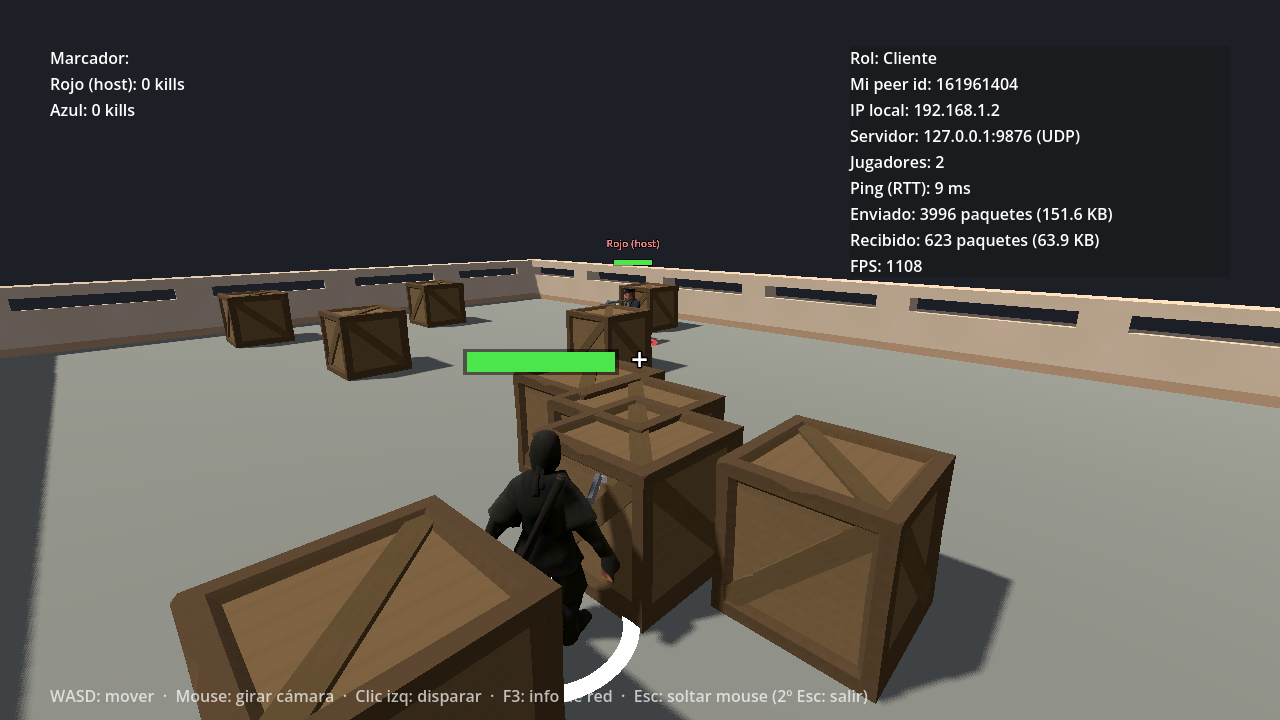
\includegraphics[width=\columnwidth]{juego-cliente.png}
\caption{Vista de un cliente con el panel de red abierto. Al fondo, el jugador
del servidor.}
\label{fig:juego}
\end{figure}

\section{Simulación en Packet Tracer}
La red se construyó en Cisco Packet Tracer 9.0.1~\cite{pt} con dos routers 2911,
dos switches 2960 y cinco PC. La configuración del Router~A es la siguiente; la
del Router~B es simétrica.

{\footnotesize
\begin{verbatim}
interface GigabitEthernet0/0
 ip address 192.168.1.1 255.255.255.0
 no shutdown
interface GigabitEthernet0/1
 ip address 10.0.0.1 255.255.255.252
 no shutdown
ip route 192.168.2.0 255.255.255.0 10.0.0.2
\end{verbatim}
}

La tabla de enrutamiento del Router~A confirma la ruta estática (S) hacia la
LAN~B:

{\footnotesize
\begin{verbatim}
C 10.0.0.0/30 is directly connected, Gi0/1
C 192.168.1.0/24 is directly connected, Gi0/0
S 192.168.2.0/24 [1/0] via 10.0.0.2
\end{verbatim}
}

\section{Pruebas y resultados}
\subsection{Conectividad en la simulación}
Desde cada uno de los cuatro PC cliente se hizo ping al servidor. En todos se
recibieron las cuatro respuestas, sin pérdida, y con TTL~126. Como el TTL
inicial es 128, los paquetes atravesaron dos routers. El primer ping después de
encender la red perdió dos paquetes mientras se resolvía ARP en cada salto, lo
cual es normal.

La orden \texttt{tracert} muestra el camino completo, con los tres saltos
esperados:

{\footnotesize
\begin{verbatim}
C:\>tracert 192.168.1.10
  1   0 ms   0 ms   0 ms   192.168.2.1
  2   0 ms   0 ms   0 ms   10.0.0.1
  3   0 ms   0 ms   0 ms   192.168.1.10
\end{verbatim}
}

El ping en sentido contrario, del servidor a un cliente, también respondió sin
pérdida. Packet Tracer no ejecuta el juego, pero demuestra que existe
conectividad IP de extremo a extremo y que ningún equipo filtra el puerto UDP
9999, que es lo que el juego necesita.

\subsection{Prueba funcional del juego}
El juego se probó con un servidor y cuatro clientes ejecutándose en un mismo
equipo, conectados por ENet, la misma cantidad de equipos de la simulación. Los
cinco procesos vieron a los cinco jugadores y el mismo marcador. También se
comprobó que el servidor calcula el movimiento de los jugadores, que las balas
creadas en el servidor aparecen en los clientes y que el daño y las
eliminaciones se registran. La Tabla~\ref{tab:medidas} recoge los valores del
panel de red de un cliente durante una prueba corta con dos jugadores
(Fig.~\ref{fig:juego}).

\begin{table}[htbp]
\caption{Mediciones en un cliente (mismo equipo)}
\label{tab:medidas}
\centering
\begin{tabular}{|l|c|}
\hline
\textbf{Medida} & \textbf{Valor} \\
\hline
Latencia de ida y vuelta (RTT) & 9 ms \\
Paquetes enviados & 3996 (151,6 KB) \\
Paquetes recibidos & 623 (63,9 KB) \\
\hline
\end{tabular}
\end{table}

El cliente envía muchos más paquetes de los que recibe porque manda su entrada
en cada cuadro dibujado, y en la prueba el juego corría a más de 1000 cuadros
por segundo. Los paquetes son pequeños, de unos 38 bytes en promedio. Una mejora
directa es enviar la entrada a una frecuencia fija, por ejemplo 60 veces por
segundo.

\subsection{Prueba con equipos físicos}
\textbf{[PENDIENTE: completar después de la prueba con los dos routers reales.
Incluir el modelo de los routers, la latencia (RTT) mostrada por el panel F3, el
resultado de ping y tracert desde un cliente y una foto del montaje.]}

\section{Conclusiones}
La arquitectura cliente-servidor con servidor autoritativo resultó adecuada para
el juego: todos los jugadores ven el mismo estado y el cliente se limita a
enviar entradas y a dibujar.

UDP, usado por medio de ENet, permitió separar el tráfico según su necesidad:
los datos que se renuevan de forma continua viajan sin garantía de entrega y los
eventos importantes en modo fiable.

Para que el juego funcione entre dos redes locales solo hace falta conectividad
IP entre los clientes y el servidor. En la topología LAN--WAN--LAN esto se logró
con una ruta estática en cada router, y la simulación lo confirmó con pings sin
pérdidas desde los cuatro clientes y un \texttt{tracert} de tres saltos.

Usar como servidor el equipo de uno de los jugadores evitó montar un servidor
dedicado y mantuvo todo el sistema dentro de la red local.

La medición de tráfico mostró que la frecuencia de envío de la entrada depende
de la velocidad de dibujo del cliente, un aspecto que conviene limitar en una
versión futura.

\begin{thebibliography}{00}
\bibitem{kurose} J. F. Kurose y K. W. Ross, \emph{Computer Networking: A
Top-Down Approach}, 8.ª ed. Pearson, 2021.
\bibitem{fiedler} G. Fiedler, ``What every programmer needs to know about game
networking,'' Gaffer On Games, 2010. [En línea]. Disponible en:
\url{https://gafferongames.com}
\bibitem{rfc768} J. Postel, ``User Datagram Protocol,'' RFC 768, ago. 1980.
\bibitem{enet} L. Salzman, ``ENet: Reliable UDP networking library.'' [En
línea]. Disponible en: \url{http://enet.bespin.org}
\bibitem{rfc1918} Y. Rekhter, B. Moskowitz, D. Karrenberg, G. J. de Groot y E.
Lear, ``Address Allocation for Private Internets,'' RFC 1918, feb. 1996.
\bibitem{godot} Godot Engine, ``High-level multiplayer,'' documentación de
Godot 4. [En línea]. Disponible en: \url{https://docs.godotengine.org}
\bibitem{pt} Cisco Networking Academy, ``Cisco Packet Tracer.'' [En línea].
Disponible en: \url{https://www.netacad.com}
\end{thebibliography}

\end{document}
